\begin{frame}{semi-supervised audio classification}{introduction}
\begin{itemize}
    \item   \textbf{observation}:
        \begin{itemize}
            \item unlabeled data is readily available 
                \begin{itemize}
                    \item example: OpenMIC dataset (musical instrument classification)
                        \begin{figure}%
                            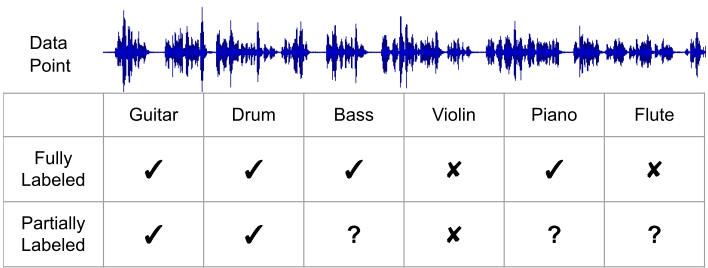
\includegraphics[scale=.3]{openmic}%
                        \end{figure}
                \end{itemize}
        \end{itemize}
    \bigskip
    \item<2->  \textbf{goal}: 
        \begin{itemize}
            \item utilize \textit{unlabeled} data for training to improve inference
        \end{itemize}
\end{itemize}
\end{frame}

\begin{frame}{semi-supervised audio classification}{experimental setup: data}
    \begin{columns}
        \column{.6\linewidth}
            \begin{itemize}
                \item   OpenMic:
                    \begin{itemize}
                        \item   20 classes of musical instruments
                        \item   \unit[10]{s} audio snippets (20000)
                        \item   90\% of labels are missing
                    \end{itemize}
                \bigskip
                \item   SONYC Urban Sound Tagging:
                    \begin{itemize}
                        \item   23 classes of urban noise
                        \item   \unit[10]{s} audio snippets ($13538+4308+669$)
                        \item   6\% of labels are missing
                    \end{itemize}
            \end{itemize}
        \column{.4\linewidth}
            \begin{figure}%
                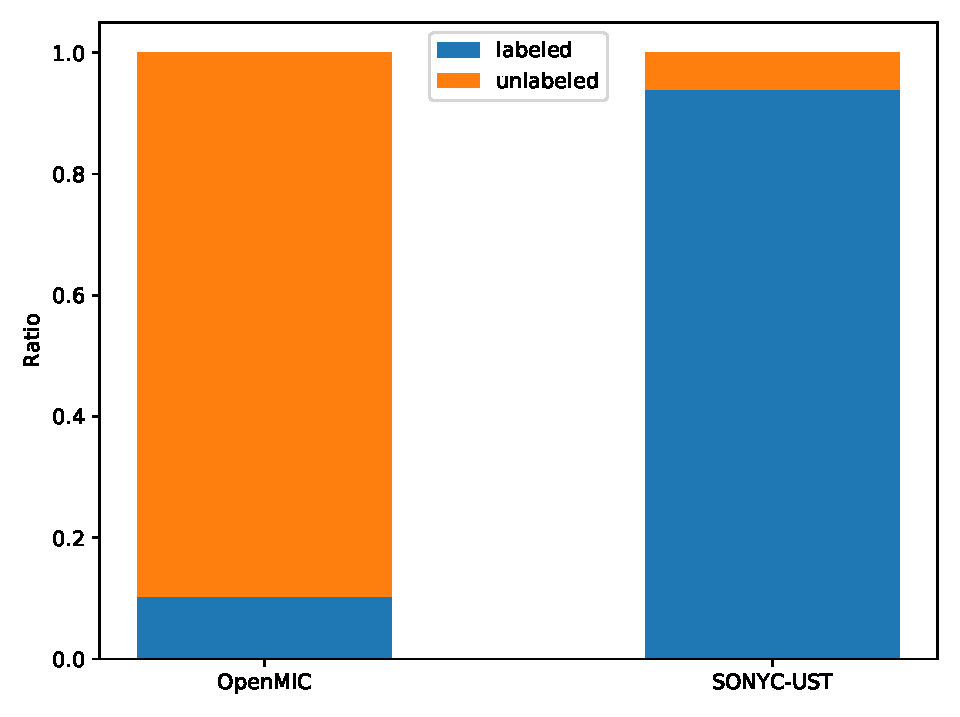
\includegraphics[scale=.3]{dataset}%
            \end{figure}
    \end{columns}
\end{frame}

\begin{frame}{semi-supervised audio classification}{experimental setup: baselines}
    \begin{itemize}
        \item Baseline 0 (B0):
            \begin{itemize}
                \item   missing labels are treated as negative labels
                \item   ``standard approach''
            \end{itemize}
        \bigskip
        \item   Baseline 1 (B1):
            \begin{itemize}
                \item   missing labels are masked out of the loss function
            \end{itemize}
    \end{itemize}
\end{frame}

\begin{frame}{semi-supervised audio classification}{method 1: label enhancing}
    \begin{columns}
        \column{.6\linewidth}
            \begin{itemize}
                \item   stage 1: 
                    \begin{itemize}
                        \item   assume all missing labels are negative 
                        \item train a teacher system
                    \end{itemize}
                \bigskip
                \item   stage 2: 
                    \begin{itemize}
                        \item   predict labels with teacher
                        \item   train student with combined training set/likely predicted labels
                        \item   mask the loss for unlikely negatives
                    \end{itemize}
            \end{itemize}
        \column{.4\linewidth}
            \begin{figure}%
                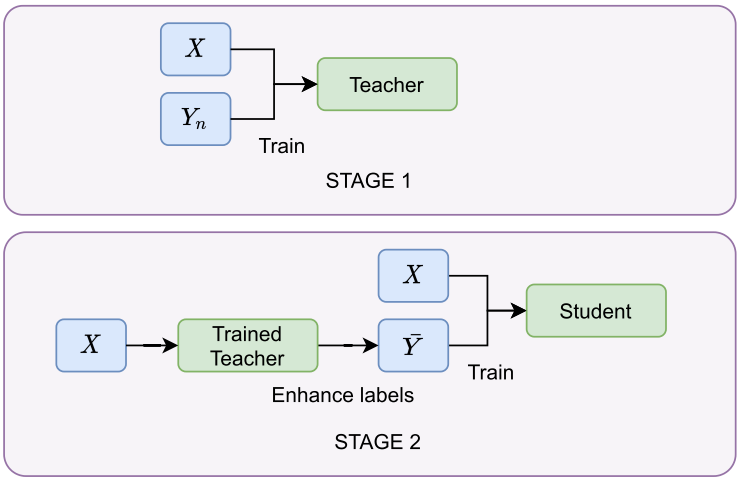
\includegraphics[scale=.3]{labelenhancing}%
            \end{figure}
    \end{columns}
    \phantom{\footfullcite{fonseca_addressing_2020}}
\end{frame}

\begin{frame}{semi-supervised audio classification}{method 2: mean teacher}
    \begin{columns}
        \column{.6\linewidth}
            \begin{itemize}
                \item   teacher and student are trained simultaneously
                \bigskip
                \item   teacher is exponential average (EMA) of student
                \bigskip
                \item   consistency loss is computed from the teacher predictions
                \bigskip
                \item   student is updated with both consistency loss and binary cross-entropy loss
            \end{itemize}
        \column{.4\linewidth}
            \begin{figure}%
                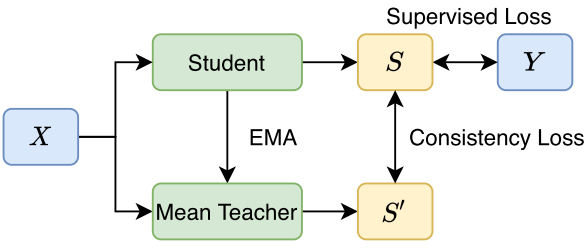
\includegraphics[scale=.3]{meanteacher}%
            \end{figure}
    \end{columns}
    \phantom{\footfullcite{bachman_learning_2014}}
\end{frame}

\begin{frame}{semi-supervised audio classification}{results: classification}
    \vspace{-5mm}
    \begin{columns}
        \column{.5\linewidth}
            \begin{itemize}
                \item   general observations
                    \begin{itemize}
                        \item B0 always worse performance
                        \item B1 much better but can be outperformed
                    \end{itemize}
                \bigskip
                \item[  (i)]   OpenMic:
                    \begin{itemize}
                        \item   Mean Teacher outperforms Label Enhancing
                    \end{itemize}
                \bigskip
                \item[(iii)]   SONYC Urban Sound Tagging:
                    \begin{itemize}
                        \item   comparable performance of Mean Teacher and Label Enhancing
                    \end{itemize}
            \end{itemize}
        \column{.5\linewidth}
            \begin{figure}%
                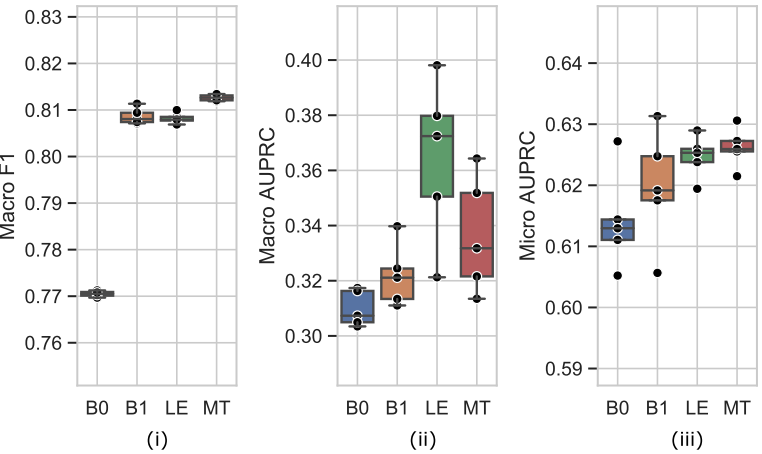
\includegraphics[scale=.3]{semi-results}%
            \end{figure}
    \end{columns}
    \phantom{\footfullcite{gururani_semi-supervised_2021}}
\end{frame}

\begin{frame}{semi-supervised audio classification}{results: data dependency}
    \begin{columns}
        \column{.5\linewidth}
            \begin{itemize}
                \item   removing labels from SONYC Urban Sound Tagging
                    \begin{itemize}
                        \item baselines deteriorate much faster
                    \end{itemize}
            \end{itemize}
        \column{.5\linewidth}
            \begin{figure}%
                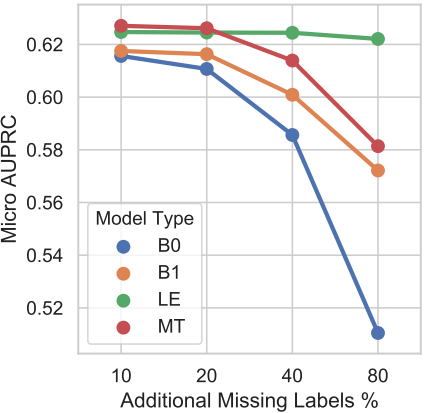
\includegraphics[scale=.45]{semi-results-data}%
            \end{figure}
    \end{columns}
    \phantom{\footfullcite{gururani_semi-supervised_2021}}
\end{frame}
